\label{sec:simulation}

\begin{figure}[h!]
\centering
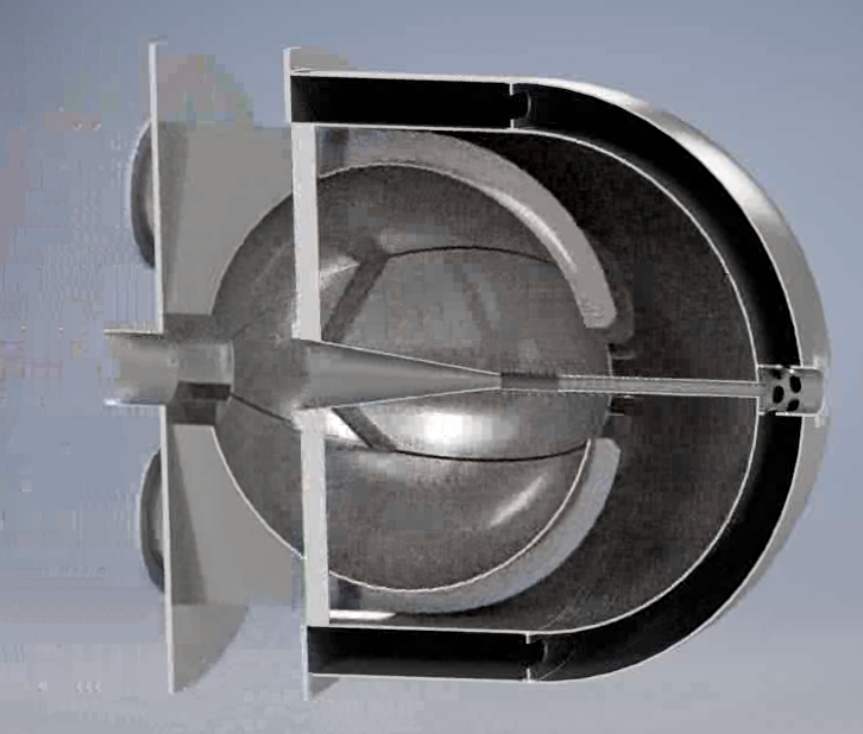
\includegraphics[width=.4\textwidth]{sections/figures/calo.Xe.png}
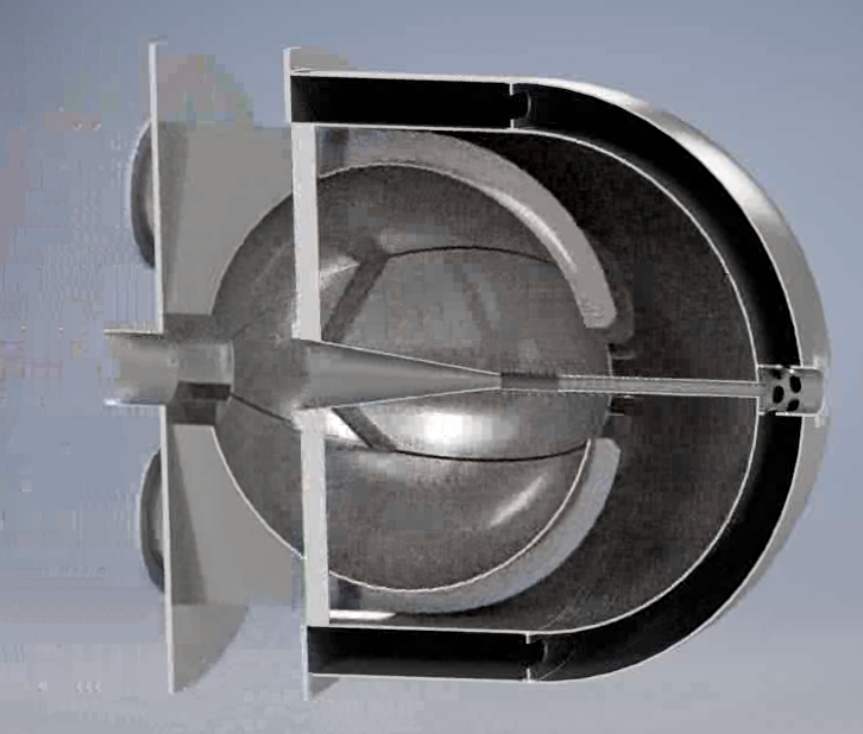
\includegraphics[width=.4\textwidth]{sections/figures/calo.Xe.png}
\caption{Left: A view of the active target system, showing the alternating planes. Right: A view of the full simulation,showing the calo }
\label{fig:simulation.view}
\end{figure}

A Monte Carlo simulation of the ATAR and CALO systems, based on the Geant4 simulation toolkit \cite{geant4}, has been undertaken in recent weeks. The simulated ATAR consists of 50 planes of 100 silicon strips, with the orientation of the strips within each plane rotated 90$^\circ$ with respect to its neighbours. Each strip has a $200 \mu m$ pitch and $120 \mu m$ thickness, giving our target an overall size of $20 mm \times 20 mm \times 6 mm$. Each strip can be read out separately in the simulation, allowing us to track particles as they move and decay within the target. A pure $\pi^{+}$ beam with a momentum spread of $72.84MeV \pm 0.01023$\% is situated upstream of the target. A degrader consisting of plastic scintillator is situated immediately upstream of the target, and its thickness of $7.5 mm$ was tuned such that beam pions are stopped in the center of the ATAR. Surrounding the ATAR and degrader is a carbon fiber beampipe, which acts as a low-Z window for positrons entering the CALO volume. The simulated volume of the CALO system consists of a $80 cm$ LXe sphere with a $17^{\circ}$ cone removed upstream of the ATAR for beam focusing and a $5 cm$ cylindrical cutout for the target and beampipe. Energy deposited in the CALO can be read out both through Geant4 truth information and by counting the scintillation photons which reach the outer radius of the detector.

Because of the lack of dead volume within the ATAR, as we can expect for AC-LGADs of this thickness, each particle leaves a distinctive track and energy signature. These signatures are not only useful for tagging decays of interest, but also supress our most common sources of background: decays in flight.